\documentclass{beamer}

\usepackage{default}
\usepackage{graphicx}
\usepackage[utf8x]{inputenc}
\usepackage{amsmath}
\usepackage{amsfonts}
\usepackage{amssymb}
\usepackage{geometry}
%\usepackage{movie15}
\usepackage{media9}
%\usepackage{subfigure}
\usepackage{graphicx}
\usepackage{comment}
\usepackage{textpos}
\usepackage[spanish,es-nodecimaldot]{babel}
\usepackage{chemmacros}
\chemsetup{
formula = chemformula,
modules = thermodynamics,
modules = reactions
}
\usepackage{pict2e}
\usepackage{epstopdf}
\newcommand{\gnuplotexe}{/opt/local/bin/gnuplot}
\usepackage[shell]{gnuplottex}
\usepackage{verbatim}
\usepackage{listings}
\lstset{language=C++%
,basicstyle=\tiny\ttfamily%
,backgroundcolor=\color{black!20}%
,breaklines=true%
,keywordstyle=\bfseries\color{magenta!90}%
,commentstyle=\itshape\color{green!40!black}%
,identifierstyle=\color{black}%
,stringstyle=\color{red!95!black}%
,numbers=left%
,numberstyle=\tiny%
,identifierstyle=\color{black}%
%,title=\lstname%
}
%%%%%%%%%%%%%%%%%%%%%%%%%%%%%%%%%%%%%%%%%%%%%%%%%%%%%%%
%%%%%%%%%%%%%%%%%%%%%%%%%%%%%%%%%%%%%%%%%%%%%%%%%%%%%%%
%%%%%%%%%%%%%%%%%%%%%%%%%%%%%%%%%%%%%%%%%%%%%%%%%%%%%%%
\newcommand{\currentWeek}{00}
%%%%%%%%%%%%%%%%%%%%%%%%%%%%%%%%%%%%%%%%%%%%%%%%%%%%%%%
%%%%%%%%%%%%%%%%%%%%%%%%%%%%%%%%%%%%%%%%%%%%%%%%%%%%%%%
%%%%%%%%%%%%%%%%%%%%%%%%%%%%%%%%%%%%%%%%%%%%%%%%%%%%%%%
\usetheme{Ilmenau}

\titlegraphic{\begin{textblock}{3}(-0.9,-4.0)
     
\includegraphics[height=2.0cm, width=2.0cm]{images/buap02}
   \end{textblock}
     \begin{textblock}{3}(11.4,-4.0)
     
\includegraphics[height=2.0cm, width=2.0cm]{images/fcq}
   \end{textblock}}
	\title[FCQ-BUAP]{Desarollo de software científico para el cálculo especializado de entalpías de formación}
	\author[Édgar García Juárez]
{
\textbf{T  E  S  I  S}
}
\institute[]
{  
  	Para obtener el grado de Licenciado en Química\\[0.3cm]
  	Presenta: \\
 	 \textbf{Édgar García Juárez} \\[0.5cm]
 	 Director y Asesor:\\
	\textbf{Dr. Juan Manuel Solano Altamirano}\\ 
	\textbf{Dr. Julio Manuel Hernández Pérez}\\ 
}
	\date{27 de octubre de 2022}



\begin{document}
\setbeamertemplate{page number in head/foot}[totalframenumber]
\setbeamertemplate{navigation symbols}{}
\frame{
\titlepage
}
\frame{\tableofcontents}

%*************************************************************
\section{Introducción}
%*************************************************************
%++++++++++++++++++++++++++++++++++++++++++++++++++++++++
\begin{frame}[fragile]
\frametitle{Química computacional}
	\begin{comment}
	Uno de los grandes logros de la comunidad científica en el siglo XX fue la creación de las computadoras. Actual-
mente, el uso de la computadora en las ciencias es fundamental, al grado que el desarrollo del
cómputo creó una nueva rama de la química, la química computacional.

En la naturaleza y en el entorno científico, existen compuestos tan reactivos que no pue-
den aislarse, por lo que no pueden estudiarse mediante técnicas comunes de laboratorio. Sin
embargo, este tipo de moléculas sí pueden estudiarse con métodos computacionales. Desde
luego, no debe considerase a la química computacional como rival de las técnicas experi-
mentales tradicionales, sino como aliada, ya que cuando se utilizan ambas, se logran resul-
tados que serían imposibles de obtener si se utilizasen de forma excluyente. Podemos decir,
entonces, que la química computacional es una disciplina que comprende los aspectos de la
investigación en química que se benefician de la aplicación de las computadoras.
	\end{comment}

Las simulaciones efectuadas por computadoras tienen múltiples ventajas:
	\vspace{1cm}
	\begin{itemize}
\item Son más ecónomicas que los experimentos físicos.
\item Pueden resolver múltiples problemas.
	\end{itemize}
\end{frame}

%...................................................
%++++++++++++++++++++++++++++++++++++++++++++++++++++++++
%++++++++++++++++++++++++++++++++++++++++++++++++++++++++
%...................................................
\begin{frame}[fragile]
\frametitle{Importancia de las funciones termodinámicas}

Dentro de las magnitudes más relevantes que pueden determinarse con cierta facilidad,
empleando cálculos de estructura electrónica se encuentra la entalpía. La entalpía es usada en procesos industriales y en el estudio de la reactividad química.

\end{frame}

\begin{comment}
A la cantidad de energía de un sistema que se encuentra a presión constante se le conoce como entalpía (H).Un proceso particularmente importante, que es usado para tabular datos termoquímicos, es la formación de un compuesto a partir de sus elementos que lo conforman. A este proceso se le denomina \textbf{entalpía de formación} y es la energía involucrada en la reacción química que relaciona la formación de 1 mol de un compuesto a partir de sus elementos en su forma más estable a $p$ = 1 bar y una temperaratura dada.
\end{comment}

%...................................................
%++++++++++++++++++++++++++++++++++++++++++++++++++++++++
%++++++++++++++++++++++++++++++++++++++++++++++++++++++++
%...................................................
\begin{frame}[fragile]
\frametitle{Calorimentría y cálculos \textit{ab initio}}

\begin{figure}
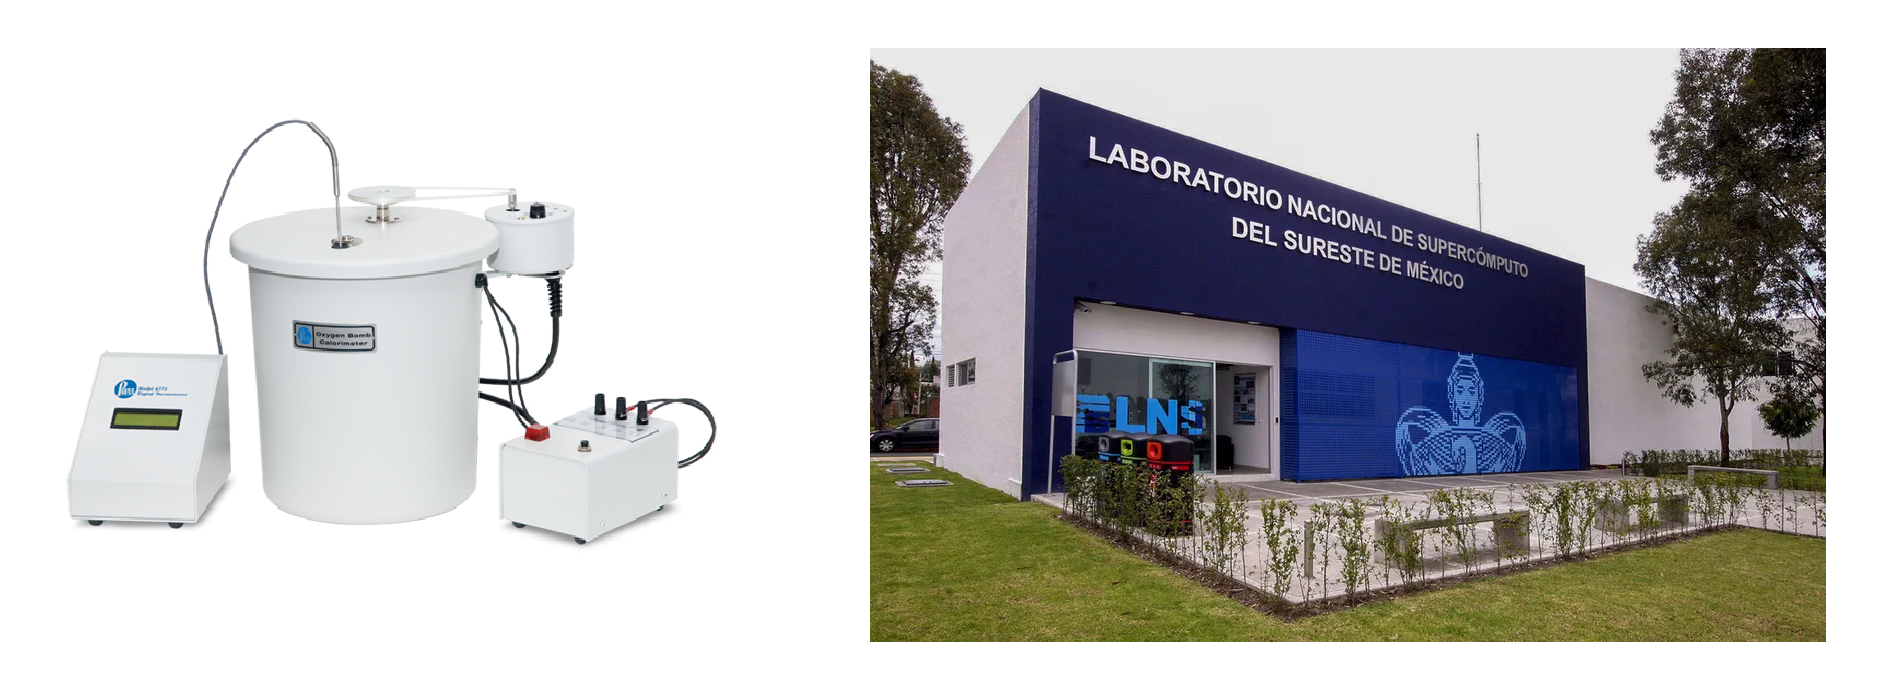
\includegraphics[scale=.28]{images/LNS.png}
\caption{Bomba calorimétrica de oxígeno y Laboratorio de supercómputo.}
\end{figure}
\begin{comment}
Una forma experimental común de determinar la $\enthalpy*(f){}$ consiste en quemar un compuesto dentro de una bomba calorimétrica y cuantificar el cambio de temperatura,
con el fin de medir la cantidad de calor involucrado en esa reacción. Teóricamente, es posible obtener la entalpía de formación haciendo uso de tablas (existen extensas tablas de entalpías de formación determinadas experimentalmente  \cite{NIST1998, Tajti2004}). No obstante, también es posible cuantificar la entalpía de formación mediante cálculos \textit{ab initio}  \cite{Lewars2016}.
Esta última opción es valiosa porque (1) es mucho más sencillo y económico que hacer un experimento termoquímico, (2) existen compuestos que no han sido medidos ni tabulados y (3) hay compuestos que son altamente reactivos, o compuestos de interés biológico que están disponibles sólo en pequeñas cantidades, por lo que no es posible someterlos a rígidos protocolos experimentales, \textit{v.gr.} reacciones de combustión.
\end{comment}
\end{frame}
%...................................................
%++++++++++++++++++++++++++++++++++++++++++++++++++++++++
%++++++++++++++++++++++++++++++++++++++++++++++++++++++++
%...................................................

\begin{frame}[fragile]
\begin{figure}
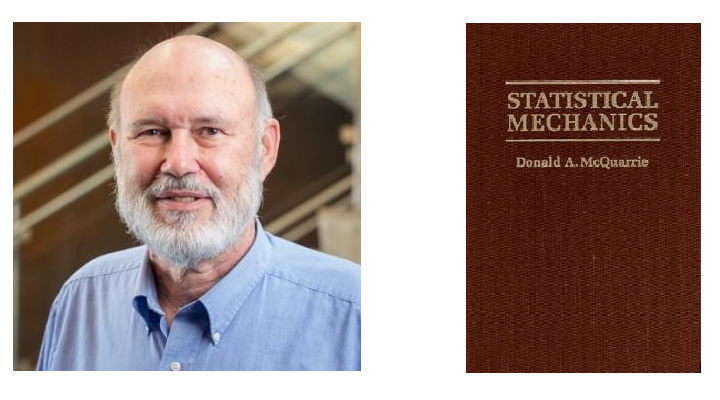
\includegraphics[scale=.7]{images/Curtis.png}
\caption{Larry A. Curtiss y mecánica estadística.}
\end{figure}
\begin{comment}
En química computacional la precisión de un cálculo computacional, en particular en la energía, varía notablemente con el nivel de teoría y con el tipo de base utilizados para realizar el cálculo.
Afortunadamente, existen metodologías que permiten conocer la energía con una precisión de
hasta $\pm$ 1 $\mathrm{cal\cdot mol^{-1}}$, respecto a una determinación experimental. Estos métodos constan de secuencias
de cálculos predefinidos y fueron desarrollados específicamente para lograr valores muy precisos
con costos computacionales aceptables (véase p. ej. los métodos introducidos por Pople \textit{et al.}\cite{Cuevas2003}). Una categoría muy popular de estos métodos combinados es la que está
conformada por las denominadas teorías \textit{Gaussian-n.}
Éstas se usan para calcular energías en sistemas moleculares que contienen átomos desde
el hidrógeno hasta el cloro, y su objetivo es desarrollar procedimientos generales,
de amplia aplicabilidad para cualquier molécula, y ser capaces de reproducir valores
termoquímicos experimentales con la precisión mencionada anteriormente.
Algunos de esos métodos son: Gn (G1, G2, G3, G4).  Existen otras técnicas como CBS-N(CBS-APNO y CBS-QB3), pero en este proyecto trabajamos exclusivamente los métodos G3 y G4 del software \textbf{Gaussian09} \cite{g09}.
\end{comment}
\end{frame}
%...................................................
%++++++++++++++++++++++++++++++++++++++++++++++++++++++++
%++++++++++++++++++++++++++++++++++++++++++++++++++++++++
%...................................................
\begin{frame}[fragile]
\frametitle{Método de atomización}
\begin{figure}
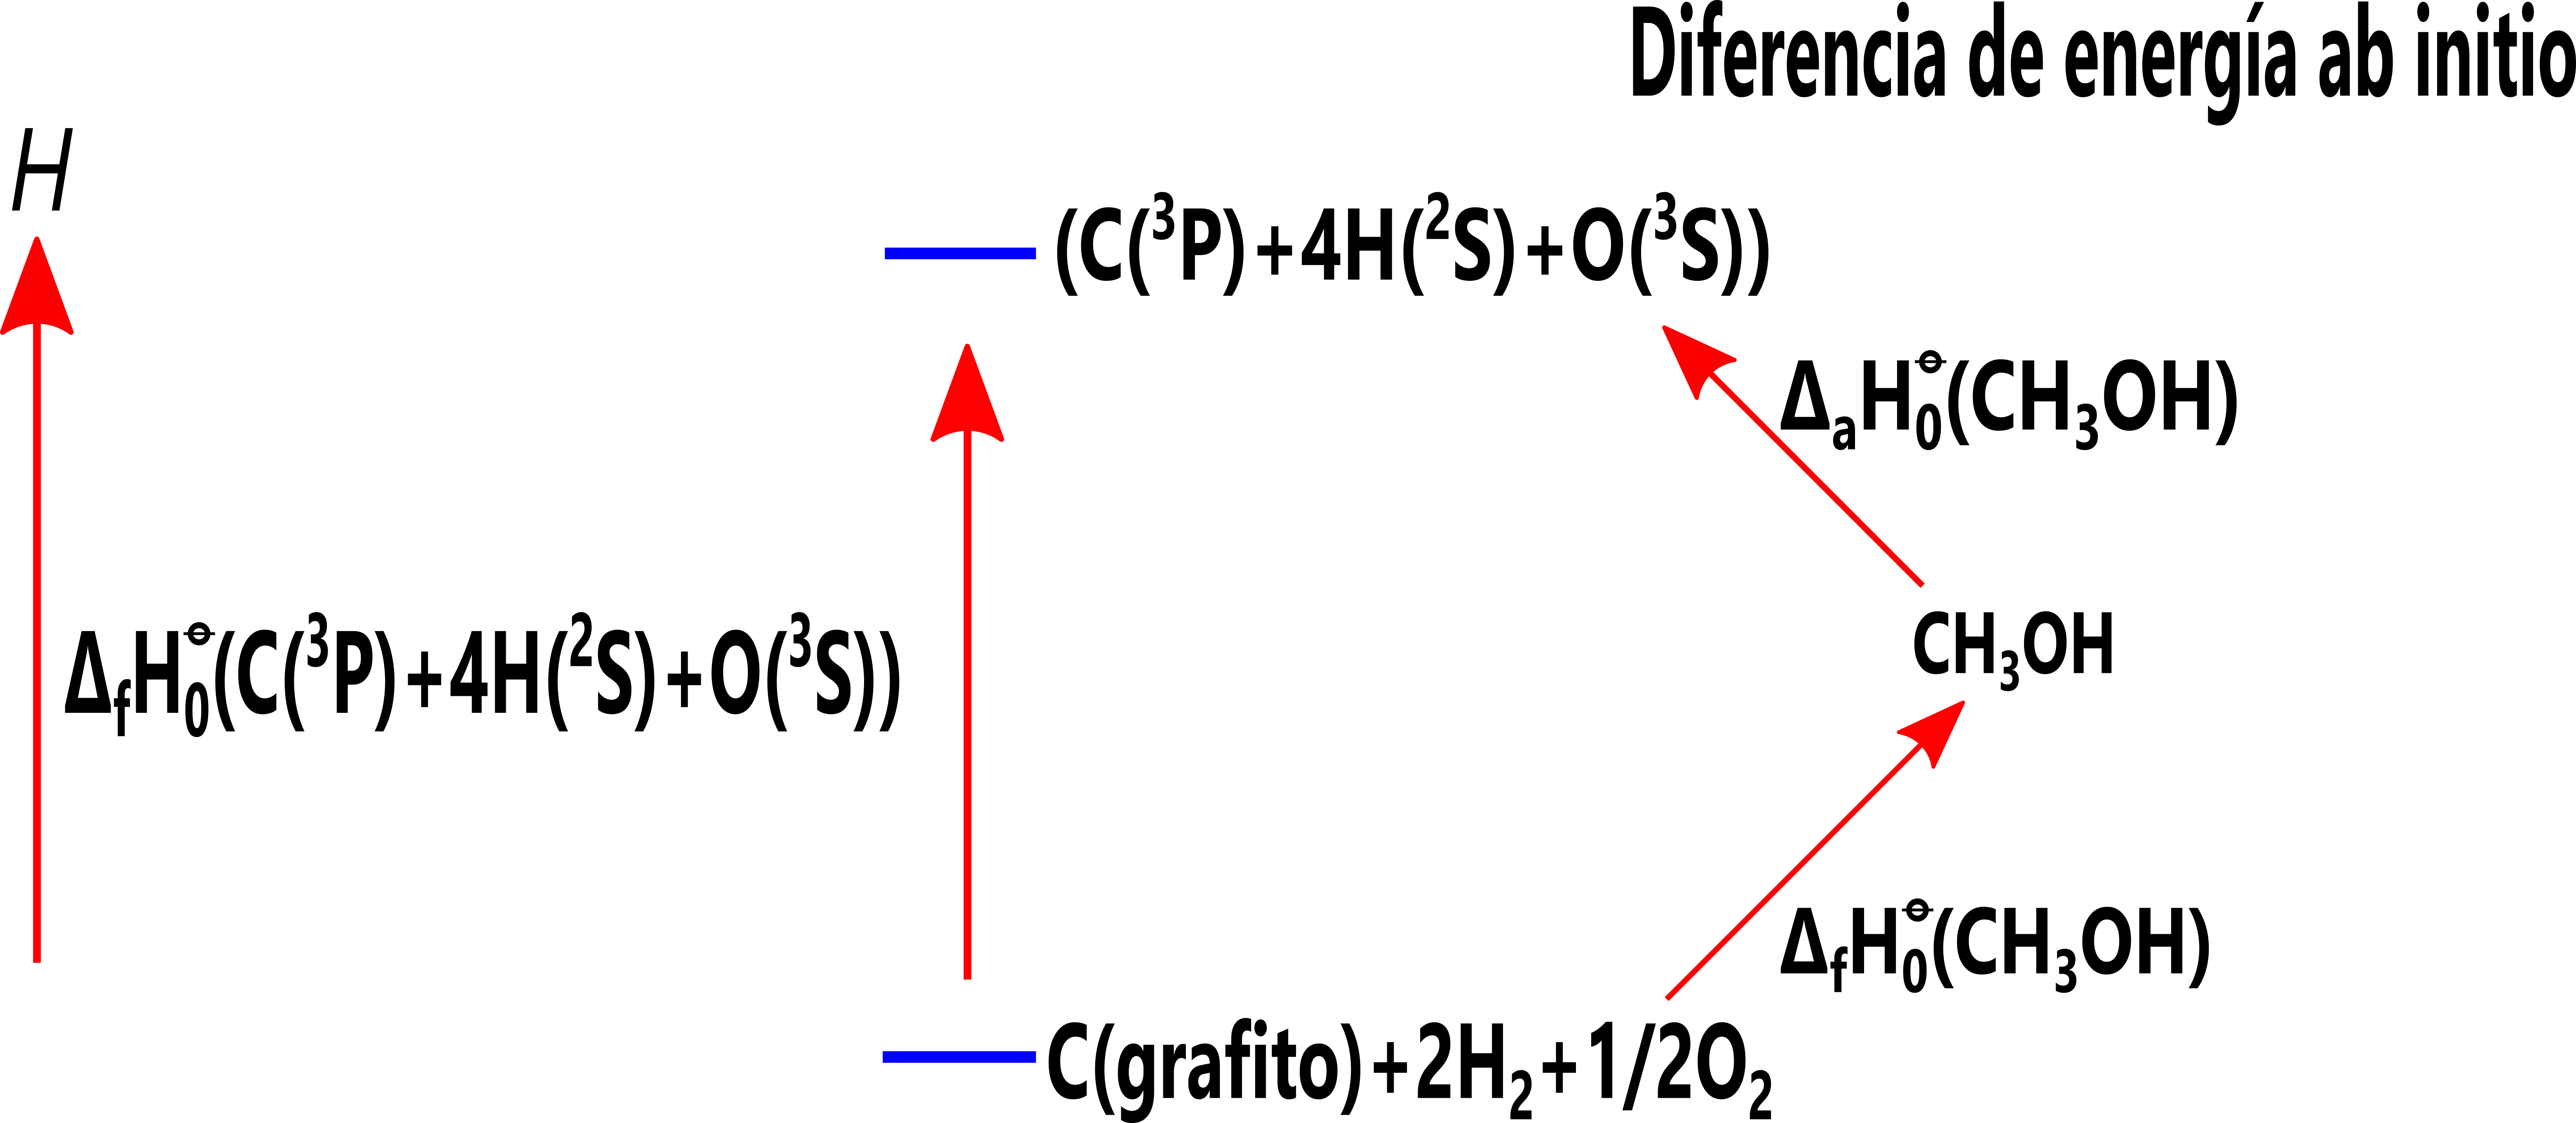
\includegraphics[scale=.65]{images/atomization-CH3OH}
\end{figure}
\tiny{\textit{Errol Lewars. Computational chemistry: introduction to the theory and applications of molecular and quantum mechanics. Springer, 2016.}}
\begin{comment}
El método G4 es un procedimiento que ha sido empleado frecuentemente en el cálculo de energías de enlace, entalpías de formación, potenciales de ionización y afinidades electrónicas. Una vez conocida la energía molecular, se puede calcular la entalpía de formación de la molécula en cuestión a  \textit{T} = 0. Para esto, se puede utilizar algunos de los tres enfoques más comúnes: el método de atomización, el método de formación o  el método de reacción isodésmica. De los tres enfoques anteriores, el método de atomización da mejores resultados, especialmente para moléculas orgánicas, y es conceptualmente el más sencillo, ya que consiste en romper
los enlaces de la molécula para obtener a sus átomos en fase gasesosa. 
\end{comment}
\end{frame}
%...................................................
%++++++++++++++++++++++++++++++++++++++++++++++++++++++++
%++++++++++++++++++++++++++++++++++++++++++++++++++++++++
%...................................................
\begin{frame}[fragile]
\frametitle{Termodinámica estadística}
\begin{comment}
Ahora bien, es común que las entalpías de formación estén tabuladas en condiciones normales de temperatura y presión, por lo que después de obtener las energías a \textit{T} = 0, es necesario calcularlas a \textit{T} = 298 K. Esto se puede hacer mediante la Termodinámica Estadística. La Termodinámica Estadística permite obtener el valor de la energía interna de una molécula, a \textit{T} = 298 K, mediante la función de partición de un gas ideal. Podemos definir a la \textbf{energía interna} como la  energía relacionada con el movimiento aleatorio y desordenado de las moléculas, es decir, la energía interna esta formada por energías de traslación, rotación, vibración, electrónica y nuclear, así como interacciones intermoleculares. 


Y la función partición resulta ser un producto de funciones de partición relacionadas con movimientos traslacionales, rotacionales y vibracionales. El término translacional contribuye con 1/2 RT, el término rotacional aporta 3/2 RT (aunque sólo RT si la molécula es lineal). Estas cantidades son el resultado de considerar a las moléculas como si fueran partículas libres en una caja para el movimiento translacional, la aproximación del rotor rigido para el movimiento rotacional y el oscilador armónico para el movimiento vibracional. Las contribuciones electrónica y nuclear son ignoradas (es decir, la función de partición correspondiente se establece en la unidad). 


Este procedimiento suele ser bastante tedioso si se realiza manualmente, por lo que resulta indispensable contar con una herramienta que permita calcular las correcciones térmicas de manera automática. 
\end{comment}

\begin{equation}
H(T)-H(0) = \int_{0} ^{T} C_{p} dT = \frac{RT^{2}}{Q} \frac{\partial Q}{\partial T} + RT
\label{eq:3.26}
\end{equation}


\begin{equation}
Q = Q_{tras}Q_{rot}Q_{vib}Q_{elec}
\label{eq:3.27}
\end{equation}

\begin{equation}
[H(T)-H(0)]_{tras} = \mathrm{\frac{3}{2}} RT
\label{eq:3.28}
\end{equation}

\begin{equation}
[H(T)-H(0)]_{rot} = \mathrm{\frac{3}{2}} RT
\label{eq:3.29}
\end{equation}


%\begin{equation}
%[H(T)-H(0)]_{rot}^{lineal} =  RT
%\label{eq:3.30}
%\end{equation}

\begin{equation}
[H(T)-H(0)]_{vib}=RT \sum_i \left(\frac{h\nu_i}{kT}\right)\left(\frac{e^{\frac{-h\nu_i}{kT}}}{1-e^{\frac{-h\nu_i}{kT}}}\right)
\label{eq:3.31}
\end{equation}
\end{frame}

\begin{frame}[fragile]


\begin{multline}
[H(298.15)-H(0)] =... \\... [H(T)-H(0)]_{tras}+[H(T)-H(0)]_{rot}+[H(T)-H(0)]_{vib}
\end{multline}


\begin{multline}
[H(298.15)-H(0)] =... \\... \mathrm{\frac{3}{2}} RT+ \mathrm{\frac{3}{2}} RT + RT \sum_i \left(\frac{h\nu_i}{kT}\right)\left(\frac{e^{\frac{-h\nu_i}{kT}}}{1-e^{\frac{-h\nu_i}{kT}}}\right)
\end{multline}

\begin{multline}
[H(298.15)-H(0)] =... \\... \mathrm{\frac{3}{2}} RT+  RT + RT \sum_i \left(\frac{h\nu_i}{kT}\right)\left(\frac{e^{\frac{-h\nu_i}{kT}}}{1-e^{\frac{-h\nu_i}{kT}}}\right)
\end{multline}




\begin{comment}
Para calcular los incrementos de la entalpía a diferentes temperaturas se usan las ecuaciones 1, 2, 3, 4, 5  y 6. Esto es $[H(298.15)-H(0)] = [H(T)-H(0)]_{vib}+[H(T)-H(0)]_{rot}+[H(T)-H(0)]_{tras}$. La contribución electrónica es ignorada (es decir, la función de partición correspondiente se establece en la unidad). Por otra parte, es posible remplazar la diferencia de las dos cantidades Gn o CBS proporcionadas en el resumen termoquímico  implementado en \textit{Gaussian} por el valor de la entalpía (energía interna) a partir de su función de partición \cite{Irikura1998}.
\end{comment}

\end{frame}












%...................................................
%++++++++++++++++++++++++++++++++++++++++++++++++++++++++
%++++++++++++++++++++++++++++++++++++++++++++++++++++++++
%...................................................

%*************************************************************
\section{Objetivos y Justificación}
%*************************************************************

\begin{frame}{fragile}
\frametitle{Objetivos}

\begin{block}{Objetivo general}

Crear un programa de cómputo científico que determine la entalpía de formación de compuestos orgánicos a $T$ = 298 K con correcciones en la energía interna, usando archivos de salida del software Gaussian.
\end{block}

\end{frame}

%...................................................
%++++++++++++++++++++++++++++++++++++++++++++++++++++++++
%++++++++++++++++++++++++++++++++++++++++++++++++++++++++
%...................................................

\begin{frame}{fragile}
\frametitle{Objetivos}

\begin{block}{Objetivos particulares}

\begin{itemize}

\item Diseñar un algoritmo de programación que pueda utilizarse a través de la línea de comandos en un sistema operativo de GNU/Linux.
\vspace{1cm}
\item Diseñar dicho programa con un lenguaje de programación orientado a objetos, de manera que sea posible fragmentar el código en partes independientes para futuros proyectos.

\end{itemize}
\end{block}
\end{frame}
%...................................................
%++++++++++++++++++++++++++++++++++++++++++++++++++++++++
%++++++++++++++++++++++++++++++++++++++++++++++++++++++++
%...................................................
\begin{frame}{fragile}
\frametitle{Justificación}

\begin{block}{Justificación}

El desarollo de software científico de alto rendimiento en Termoquímica es una de las principales líneas de investigación de nuestro grupo de investigación. Por lo tanto, el cálculo de funciones termodinámicas de forma optimizada dará como resultado una alta eficiencia en el flujo de trabajo.
\end{block}

\end{frame}
%...................................................
%++++++++++++++++++++++++++++++++++++++++++++++++++++++++
%++++++++++++++++++++++++++++++++++++++++++++++++++++++++
%...................................................


%*************************************************************
\section{Metodología}
%*************************************************************
\begin{frame}[fragile]{Code}
\frametitle{Script}
\begin{comment}
Este script genera un archivo que se utilizará como entrada para el programa.
Nombre del programa JMHP. Se supone que el archivo de salida gaussiano corresponde
a un cálculo G4 (o cualquier Gn), y que el archivo de entrada gaussiana contenía
una matriz z. Es decir, la molécula a estudiar con un método G4 debe ser
dada en el archivo de entrada gaussiana como una matriz z.

Por lo general, 'gaussianoutfile' tiene una extensión *.out o *.log.
El script utilizará la matriz z inicial para determinar el número de átomos,
el número de diferentes especies atómicas, etc. Esta matriz z se registra
dentro del archivo de salida gaussiana.

Si no se dan opciones, los contenidos de configuración generados (la configuración
parámetros para ejecutar JMHP-ProgramName) se mostrarán en la pantalla.
\end{comment}
\begin{block}{gendeltahfinputfile}
Este script genera un archivo que se utilizará como entrada para el programa EnthalpyNIST. El archivo de salida de Gaussian corresponde a un cálculo G4 (o cualquier Gn).
\end{block}
\end{frame}
%...................................................
%++++++++++++++++++++++++++++++++++++++++++++++++++++++++
%++++++++++++++++++++++++++++++++++++++++++++++++++++++++
%...................................................
\begin{frame}
\frametitle{Diagrama de flujo 1}
\begin{center}
\begin{figure}[h!]
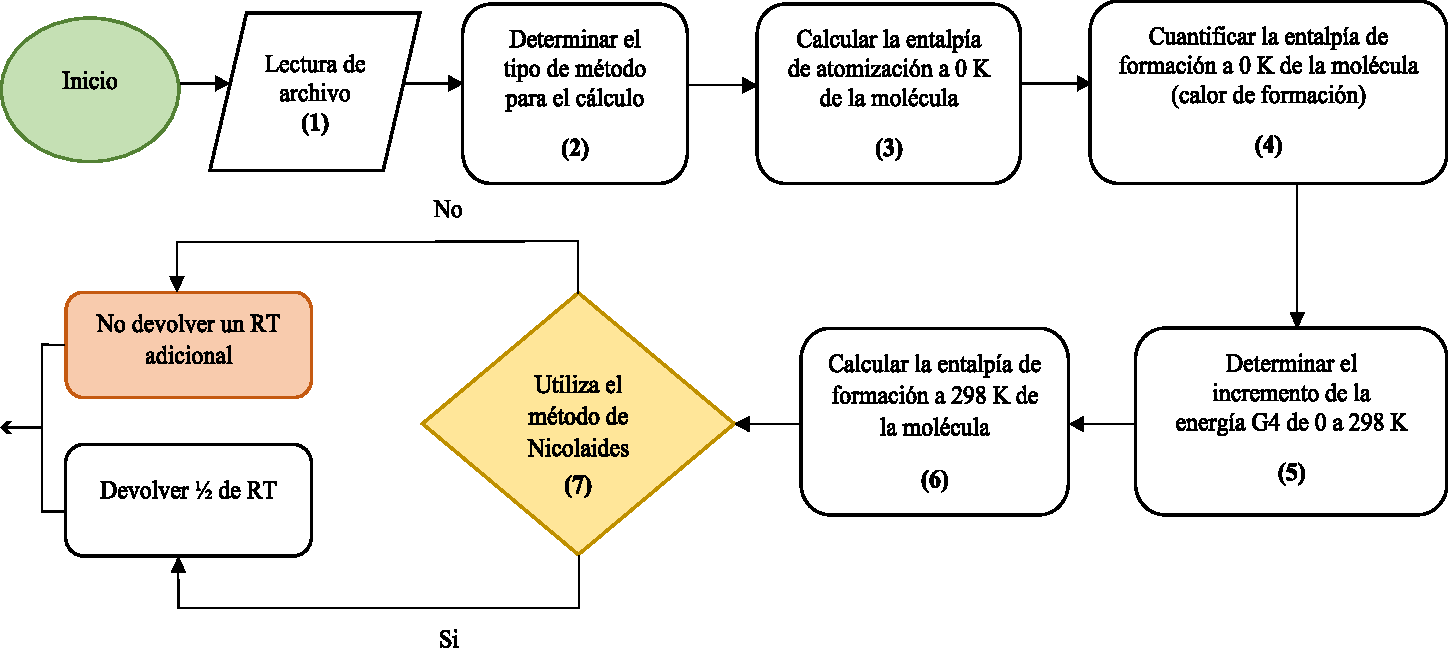
\includegraphics[scale=.45]{images/df1}
\end{figure}
\end{center}
\end{frame}
%...................................................
%++++++++++++++++++++++++++++++++++++++++++++++++++++++++
%++++++++++++++++++++++++++++++++++++++++++++++++++++++++
%...................................................
\begin{frame}
\frametitle{Diagrama de flujo 2}
\begin{center}
\begin{figure}[h!]
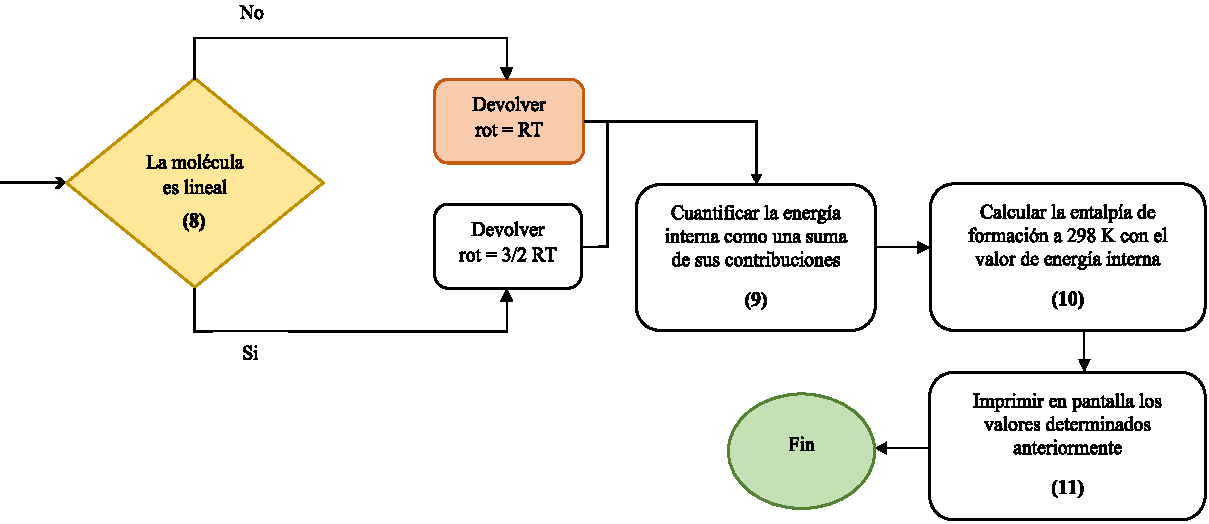
\includegraphics[scale=.55]{images/df2}
\end{figure}
\end{center}
\end{frame}
%...................................................
%++++++++++++++++++++++++++++++++++++++++++++++++++++++++
%++++++++++++++++++++++++++++++++++++++++++++++++++++++++
%...................................................
\begin{frame}

\begin{center}
\begin{figure}[h]
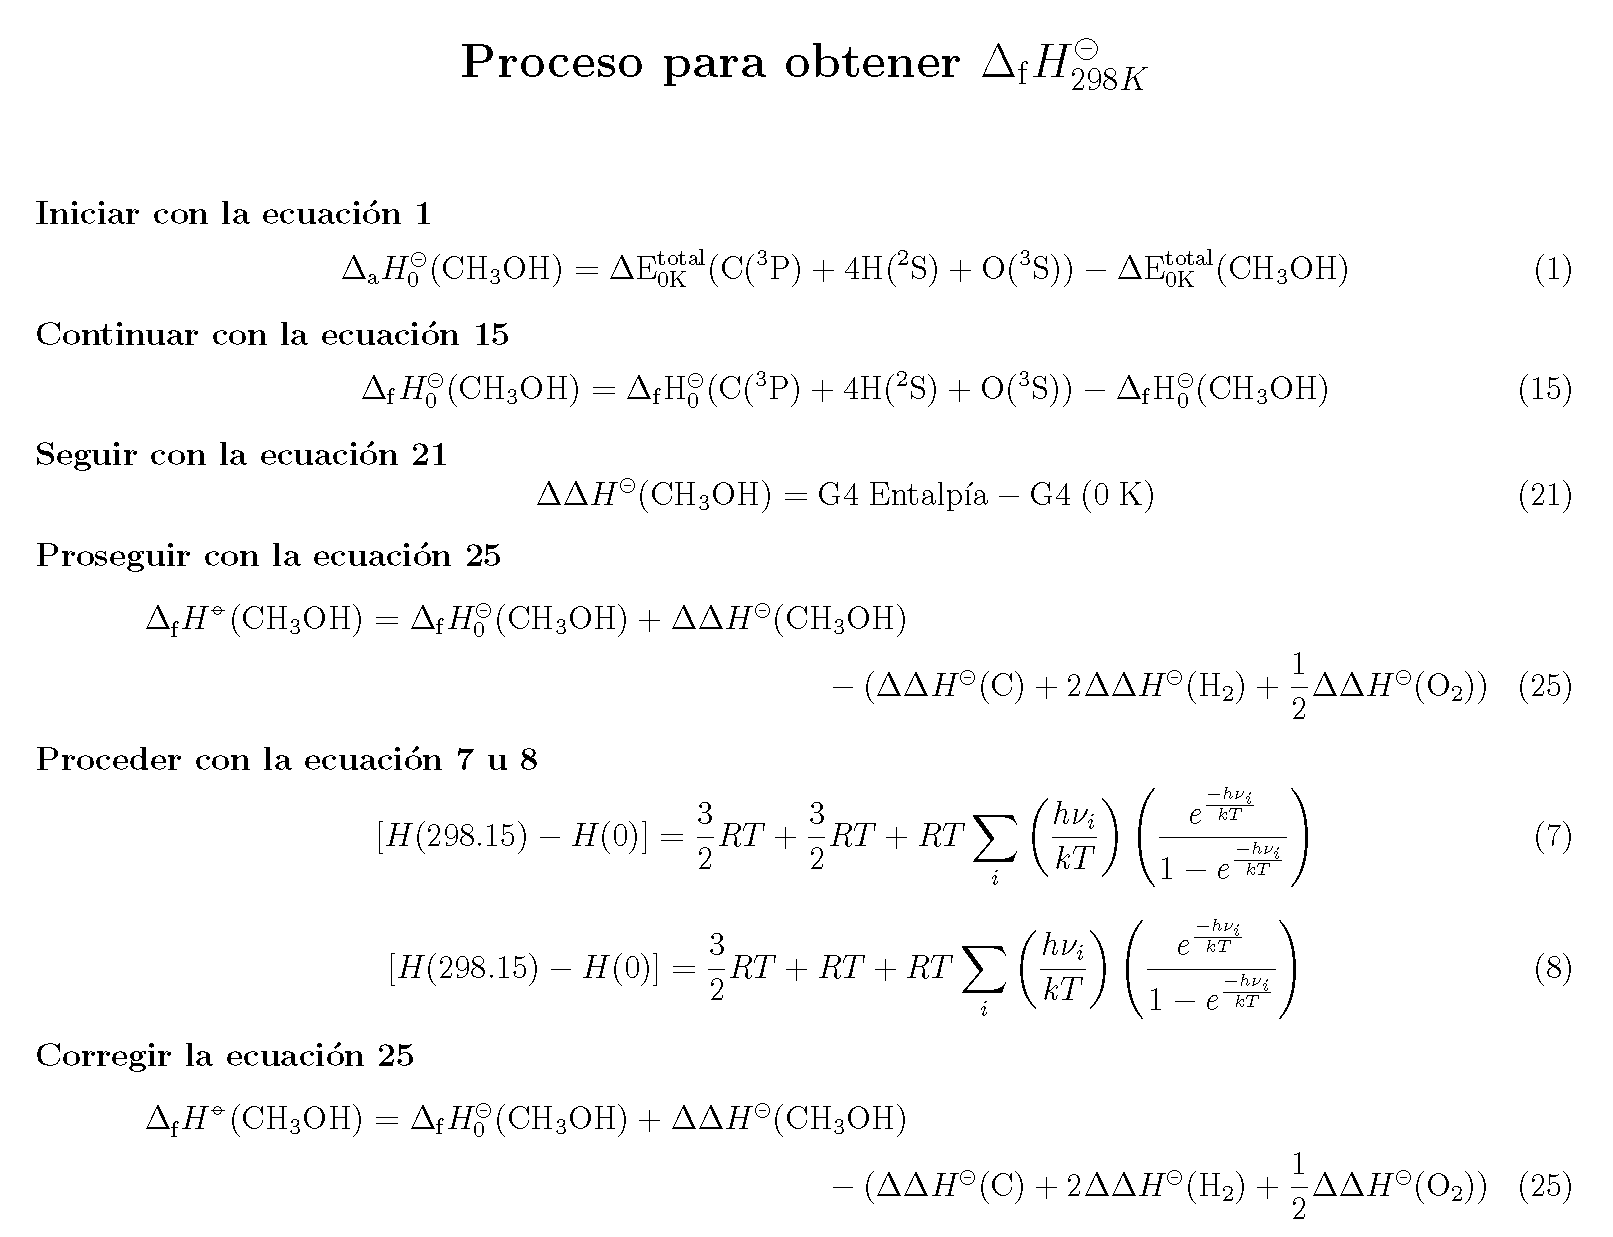
\includegraphics[scale=.3]{images/procesoH298.png}
\end{figure}
\end{center}
\end{frame}
%...................................................
%++++++++++++++++++++++++++++++++++++++++++++++++++++++++
%++++++++++++++++++++++++++++++++++++++++++++++++++++++++
%...................................................
\begin{frame}[fragile]{Code}
\frametitle{Inicio}

\begin{comment}
El programa comienza con la lectura de un archivo de entrada que contiene la información necesaria de la molécula. Para la \textbf{molécula X}, el archivo de entrada tendrá la siguiente forma:
\end{comment}

\begin{block}{Output de CH3OH-G4.txt}
\begin{lstlisting}
G4
3
-115.651767
-115.647489
1 4
6 1
8 1
0
0
12
322.7598
1058.0227
1094.4693
1175.9092
1389.4710
1487.0775
1495.0437
1513.5228
2980.0300
3023.9572
3106.3296
3831.1143
\end{lstlisting}
\end{block}
\end{frame}
%...................................................
%++++++++++++++++++++++++++++++++++++++++++++++++++++++++
%++++++++++++++++++++++++++++++++++++++++++++++++++++++++
%...................................................
\begin{frame}[fragile]{Code}
\frametitle{Paso 1: Lectura de archivo de entrada}
\begin{comment}
Ahora, se leerá el archivo de entrada de la siguiente forma:
\end{comment}
\begin{block}{Output de CH3OH-G4.txt}
\begin{enumerate}		
	\item Categoría de método. 
	\item Número de especies atómicas.
	\item Energía G4 a 0 K.
	\item Entalpía G4 a 0 K.
	\item Número atómico y número de átomos.
	\item Tipo de molécula (lineal o no lineal).
	\item Modelo de aproximación usada (Nicolaides o Rotor Rígido/Oscilador Armónico).
	\item Número de modos de vibración.
	\item Frecuencias vibracionales de la molécula.
\end{enumerate}
\end{block}
\end{frame}
\begin{comment}
Las líneas 1, 2, 3, 4 y 5 siempre se encargarán de leer la categoría del método, el número de especies atómicas, la energía G4 a $T$ = 0, la entalpía G4 a $T$ = 0, el número atómico y el número de átomos, respectivamente. Mientras que las líneas 6, 7, 8 y 9 no siempre ocuparán el mismo lugar, porque éstas dependen de líneas anteriores.\\

Por ejemplo, para la \textbf{molécula X}, el número de especies atómicas serán tres: hidrógeno, carbono y oxígeno. En consecuencia, la línea 5 se repetirá tres veces para las especies mencionadas. Después, se leerá el tipo de molécula (lineal o no lineal), posteriormente, el modelo de aproximación usada (Nicolaides o Rotor Rígido/Oscilador Armónico). Por último, el número de modos de vibración que influirá en las frecuencias vibracionales de la molécula. Al terminar el proceso de lectura, toda esta información es almacenada en variables específicas del programa. 
\end{comment}
%...................................................
%++++++++++++++++++++++++++++++++++++++++++++++++++++++++
%++++++++++++++++++++++++++++++++++++++++++++++++++++++++
%...................................................
\begin{frame}[fragile]{Code}
\frametitle{Paso 2: Selección del método}
\begin{comment}
Como segundo paso en el diagrama general, se encuentra la determinación del método uti-
lizado, que es indispensable para comenzar con los cálculos.
\end{comment}


\begin{enumerate}		
	\item G3. 
	\item G3MP2.
	\item G4.	
	\item CBS-APNO.
	\item CBS-QB3.
\end{enumerate}
\end{frame}
\begin{comment}
EnthalpyNIST, EnthalpyTajti y EnthalpyArgonne cuentan con varios los métodos...de Gaussian, pero en nuestra explicación utilizaremos el método G4 de Gaussian09. Hecho esto, el programa tiene la certeza de qué datos ocupar para las especies atómicas antes leídas.
\end{comment}
%...................................................
%++++++++++++++++++++++++++++++++++++++++++++++++++++++++
%++++++++++++++++++++++++++++++++++++++++++++++++++++++++
%...................................................

\begin{frame}[fragile]{Code}
\frametitle{Paso 3: Cálculo de la entalpía de atomización a \textit{T} = 0}
\begin{comment}
En este paso se realiza el cálculo de la entalpía de atomización a $T$ = 0 de la molécula. Aquí se utilizan los valores del método G4 para cada uno de los átomos presentes en la \textbf{molécula X}, la cantidad estequiométrica de estos y la entalpía G4 de la molécula a $T$ = 0 (veáse las ecuaciones \ref{eq:4.1} y \ref{eq:4.2}). Para concluir, se realiza una conversión de unidades de energía (hartree a kJ). Obsérvese las ecuaciones \ref{eq:4.4} y \ref{eq:4.5}.
\end{comment}


\begin{multline}
	\mathrm{\Delta}_\mathrm{{a}} H^{\circleddash}_{\mathrm{0}}\mathrm{(CH_3OH)}  = ... \\ ...\; \mathrm{\Delta} \mathrm{E^{total}_{0K}} \mathrm{(C(^{3}P)} + \mathrm{4H(^{2}S)} + \mathrm{O(^{3}S))}- \mathrm{\Delta E^{total}_{0K} (CH_{3}OH)}
\label{eq:4.1}
\end{multline}

\begin{multline}
	\mathrm{\Delta}_\mathrm{{a}} H^{\circleddash}_{0}\mathrm{(CH_3OH)} = \mathrm{-37.834170\;h} \;... \\ ...+\;\mathrm{4(-0.501420)}\;\mathrm{h - 75.045500}\;\mathrm{h -(-115.651767)\;h}
\label{eq:4.2}
\end{multline}
\end{frame}
%...................................................
%++++++++++++++++++++++++++++++++++++++++++++++++++++++++
%++++++++++++++++++++++++++++++++++++++++++++++++++++++++
%...................................................

\begin{frame}[fragile]{Code}
\frametitle{Paso 3: Cálculo de la entalpía de atomización a \textit{T} = 0}

\begin{equation}
	\mathrm{\Delta}_\mathrm{{a}} H^{\circleddash}_{0}\mathrm{(CH_3OH) = -114.88535\;\mathrm{h} + 115.651767\;\mathrm{h}}
\end{equation}

\begin{equation}
	\mathrm{\Delta}_\mathrm{{a}} H^{\circleddash}_{0}\mathrm{(CH_3OH) = (\;0.766417\;\mathrm{h})(2625.4997480\;\mathrm{kJ\;mol^{-1})}}
\label{eq:4.4}
\end{equation}

\begin{equation}
	\mathrm{\Delta}_\mathrm{{a}} H^{\circleddash}_{0}\mathrm{(CH_3OH) = 2012.22764\; \mathrm{kJ\;mol^{-1}}}
\label{eq:4.5}
\end{equation}
\end{frame}
%...................................................
%++++++++++++++++++++++++++++++++++++++++++++++++++++++++
%++++++++++++++++++++++++++++++++++++++++++++++++++++++++
%...................................................
\begin{frame}[fragile]{Code}
\frametitle{Paso 4: Cálculo de la entalpía de formación a \textit{T} = 0}
\begin{comment}
En este paso se realiza el cálculo de la entalpía de formación a $T$ = 0 de la molécula. Nuevamente, se utilizan valores experimentales para cada uno de los átomos presentes en la molécula junto con su cantidad específica y el valor de la entalpía de atomización a $T$ = 0 obtenido anteriormente (ecuaciones \ref{eq:4.6} y \ref{eq:4.7}). Al valor obtenido en este paso se le conoce como \textbf{calor de formación} (ecuación \ref{eq:4.9}). Por último, se realiza una conversión de unidades de energía (kJ a kcal), ver las ecuaciones \ref{eq:4.10} y \ref{eq:4.11}. 
\end{comment}

\begin{multline}
	\mathrm{\Delta}_\mathrm{{f}} H^{\circleddash}_{0}\mathrm{(CH_3OH)} =... \\ ...= \mathrm{\Delta_{f} H^{\circleddash}_{0}} \mathrm{(C(^{3}P) + 4H(^{2}S) + O(^{3}S))- \Delta_{f} H^{\circleddash}_{0} (CH_{3}OH)}
\label{eq:4.6}
\end{multline}

\begin{multline}
	\mathrm{\Delta}_\mathrm{{f}} H^{\circleddash}_{0}\mathrm{(CH_3OH)} = \mathrm{711.185}\;\mathrm{kJ\;mol^{-1}} +\;\mathrm{4(216.03500)}\mathrm{\;kJ\;mol^{-1}} +...\\
	+...\; \mathrm{246.7900}\;\mathrm{kJ\;mol^{-1}} - \mathrm{2012.22764}\; \mathrm{kJ\;mol^{-1}}
\label{eq:4.7}
\end{multline}

\begin{equation}
	\mathrm{\Delta}_\mathrm{{f}} H^{\circleddash}_{0}\mathrm{(CH_3OH) = 1822.115 - 2012.22764\; kJ\;mol^{-1}}
\end{equation}
\end{frame}
%...................................................
%++++++++++++++++++++++++++++++++++++++++++++++++++++++++
%++++++++++++++++++++++++++++++++++++++++++++++++++++++++
%...................................................
\begin{frame}[fragile]{Code}
\frametitle{Paso 4: Cálculo de la entalpía de formación a \textit{T} = 0}

\begin{equation}
	\mathrm{\Delta}_\mathrm{{f}} H^{\circleddash}_{0}\mathrm{(CH_3OH) = -190.11264\; kJ\;mol^{-1}}
\label{eq:4.9}
\end{equation}

\begin{equation}
	\mathrm{\Delta}_\mathrm{{f}} H^{\circleddash}_{0}\mathrm{(CH_3OH) = (-190.11264\; kJ\;mol^{-1})(0.23888\; kcal)}
\label{eq:4.10}
\end{equation}

\begin{equation}
	\mathrm{\Delta}_\mathrm{{f}} H^{\circleddash}_{0}\mathrm{(CH_3OH) = -\;45.41\;kcal}
\label{eq:4.11}
\end{equation}
\end{frame}
%...................................................
%++++++++++++++++++++++++++++++++++++++++++++++++++++++++
%++++++++++++++++++++++++++++++++++++++++++++++++++++++++
%...................................................
\begin{frame}[fragile]{Code}
\frametitle{Paso 5: Diferencia entre las  dos cantidades G4}
\begin{comment}
El paso 5 se encarga de cuantificar la diferencia entre las  dos cantidades G4 ($T$ = 0 y $T$ = 298 K) leídas en el paso 1 (ecuación \ref{eq:4.13}). Además, se realiza una conversión de unidades de energía (hartree a kJ), ecuaciones \ref{eq:4.14} y \ref{eq:4.15}.
\end{comment}

\begin{equation}
	\mathrm{\Delta \Delta} H^{\circleddash}\mathrm{(CH_3OH) = G4\;\textrm{Entalpía} - G4\;(0\;K)}
\label{eq:4.12}
\end{equation}

\begin{equation}
	\mathrm{\Delta \Delta} H^{\circleddash}\mathrm{(CH_3OH) = -115.647489\;\mathrm{h} - (-115.651767)\;h}
\label{eq:4.13}
\end{equation}

\begin{equation}
	\mathrm{\Delta \Delta} H^{\circleddash}\mathrm{(CH_3OH) = (0.004278\;\mathrm{h})(2625.4997480\; kJ\;mol^{-1})}
\label{eq:4.14}
\end{equation}

\begin{equation}
	\mathrm{\Delta \Delta} H^{\circleddash}\mathrm{(CH_3OH) = 11.23188\;kJ\;mol^{-1}}
\label{eq:4.15}
\end{equation}
\end{frame}
%...................................................
%++++++++++++++++++++++++++++++++++++++++++++++++++++++++
%++++++++++++++++++++++++++++++++++++++++++++++++++++++++
%...................................................
\begin{frame}[fragile]{Code}
\frametitle{Paso 6: Entalpía de formación a $T$ = 298 K}
\begin{comment}
En el paso 6 se obtiene el valor de la entalpía de formación a $T$ = 298 K (sumando el calor de formación, la diferencia de las dos cantidades G4 y restando los incrementos correspondientes para los elementos de la molécula en sus estados estándar), en consecuencia, se usan los valores obtenidos en los pasos 4 y 5 (veáse las ecuaciones \ref{eq:4.16}, \ref{eq:4.17}, \ref{eq:4.18} y \ref{eq:4.19}). Finalmente, se realiza una conversión de unidades de energía de kJ a kcal (ecuaciones \ref{eq:4.20} y \ref{eq:4.21}). 
\end{comment}


\begin{multline}
	\enthalpy*(f){}\mathrm{(CH_3OH)} = \mathrm{\Delta}_\mathrm{{f}} H^{\circleddash}_{0}\mathrm{(CH_{3}OH)} + \mathrm{\Delta \Delta} H^{\circleddash} \mathrm{(CH_{3}OH)}\;...\\ ...- (\mathrm{\Delta \Delta} H^{\circleddash} \mathrm{(C)} + 2 \mathrm{\Delta \Delta} H^{\circleddash}\mathrm{(H_{2})} + \mathrm{\frac{1}{2}} \mathrm{\Delta \Delta} H^{\circleddash}\mathrm{(O_{2}))}
\label{eq:4.16}
\end{multline}

\begin{multline}
	\enthalpy*(f){}\mathrm{(CH_3OH)} = \mathrm{-190.11264}\;\mathrm{kJ\;mol^{-1}} + \mathrm{11.23188}\;\mathrm{kJ\;mol^{-1}}\;...  \\ ...- \mathrm{(1.05100 + 2(8.46700) + \frac{1}{2} (8.67000))}\mathrm{\; kJ\;mol^{-1}}
\label{eq:4.17}
\end{multline}

\begin{multline}
	\enthalpy*(f){}\mathrm{(CH_3OH)} = -190.11264\;\mathrm{kJ\;mol^{-1}}\;... \\...+ 11.23188\;\mathrm{kJ\;mol^{-1}} - 22.3265\;\mathrm{\; kJ\;mol^{-1}}
\label{eq:4.18}
\end{multline}
\end{frame}
%...................................................
%++++++++++++++++++++++++++++++++++++++++++++++++++++++++
%++++++++++++++++++++++++++++++++++++++++++++++++++++++++
%...................................................
\begin{frame}[fragile]{Code}
\frametitle{Paso 6: Entalpía de formación a $T$ = 298 K}
\begin{comment}
\end{comment}

\begin{equation}
	\enthalpy*(f){}\mathrm{(CH_3OH) = -201.21\;kJ\;mol^{-1}}
\label{eq:4.19}
\end{equation}

\begin{equation}
	\enthalpy*(f){}\mathrm{(CH_3OH) = (-201.21 kJ\;mol^{-1})(0.23888 \:kcal)}
\label{eq:4.20}
\end{equation}

\begin{equation}
	\enthalpy*(f){}\mathrm{(CH_3OH) = -\;48.06 \:kcal}
\label{eq:4.21}
\end{equation}
\end{frame}
%...................................................
%++++++++++++++++++++++++++++++++++++++++++++++++++++++++
%++++++++++++++++++++++++++++++++++++++++++++++++++++++++
%...................................................
\begin{frame}[fragile]{Code}
\frametitle{Paso 7, 8 y 9: Energía interna}

\begin{comment}
Los pasos 7 y 8 son de los más importantes del programa, porque calculan la energía interna (paso 6) usando ecuaciones que provienen de la Termodinámica Estadística. Se inicia con dos sentencias de condición que evalúan parámetros de la molécula, como son:

\begin{multicols}{2}
\begin{enumerate}
	\item Aproximaciones a usar.
	\item El número de modos de vibración.
	\item Frecuencias vibracionales.
	\item Si es lineal o no.
\end{enumerate}
\end{multicols}

El tipo de aproximación usada solo puede tener dos valores, 0 y 1. Si el archivo de entrada de la molécula muestra un valor de 0 significa que se usará la aproximación de Nicolaides \textit{et al.} (no toma en cuenta las frecuencias vibraciones de la molécula menores a 260 cm$^{-1}$ y devuelve $\frac{1}{2}$ de $RT$ para la contribución vibracional por cada frecuencia que sea menor a 260 cm$^{-1}$). Y si el valor es 1, la aproximación de rotor rígido y oscilador armónico  sera usada para los cálculos. 

También existen dos posibles valores en el archivo de entrada para el parámetro de la linealidad de la molécula. Un valor de 1 devolverá un $RT$ en la contribución rotacional, en cambio, si el valor es 0, el condicional retornará un $\frac{3}{2}$ de $RT$ en la contribución rotacional. Después, se inicia una estructura de control que se repetirá el mismo número de veces que el número de modos de vibración de la molécula (una molécula que tiene $N$ especies atómicas puede tener solamente $3N-6$ modos fundamentales de vibración para una molécula no lineal, o $3N-5$ si la molécula es lineal). \\

La suma es acumulativa y son usadas las ecuaciones \ref{eq:3.27}, \ref{eq:3.28}, \ref{eq:3.29}, y \ref{eq:3.31} que provienen de la Termodinámica Estadística,para determinar a la energía interna como una suma de las contribuciones vibracionales, rotacionales, traslacionales y electrónicas (ecuación \ref{eq:3.31}). La contribuci\'{o}n traslacional siempre tendr\'{a} el valor de $\frac{3}{2} RT$ para cualquier mol\'{e}cula (ecuación \ref{eq:3.27}). Adem\'{a}s, se agrega un $RT$ adicional a la energ\'{i}a interna para convertir la energía en entalpía (el llamado término $pV$, ecuación \ref{eq:3.29}). Cabe aclarar que el valor obtenido en la primera iteración es acumulativo para los subsecuentes. Concluida la determinación, se devuelve la suma total de la energía interna. Para la \textbf{molécula X} el número de modos de vibración será 12 (es una molécula no lineal), por lo consiguiente, la ecuación \ref{eq:3.30} se repetirá 12 veces con cada una de las frecuencias de la molécula. El resultado final es la suma de las contribuciones de la energía interna, véase la ecuación \ref{eq:3.31}. 
\end{comment}

\begin{multline}
	[H(298.15)-H(0)]= 1315.1747\;\mathrm{kJ\;mol^{-1}} +\; 3718.4568\;\mathrm{kJ\;mol^{-1}}\;...\\...+\; 3718.4568\;\mathrm{kJ\;mol^{-1}} +\;2478.9712\;\mathrm{kJ\;mol^{-1}} = \mathrm{11.2310\;kJ\;mol^{-1}}
\label{eq:4.22}
\end{multline}
\end{frame}
%...................................................
%++++++++++++++++++++++++++++++++++++++++++++++++++++++++
%++++++++++++++++++++++++++++++++++++++++++++++++++++++++
%...................................................
\begin{frame}[fragile]{Code}
\frametitle{Paso 10: Remplazo de la energía interna}
\begin{comment}
El paso 10 simplemente remplaza el valor obtenido anteriormente (energía interna), por el valor calculado en el paso 5 en la determinación de la entalpía de formación a $T$ = 298 K, es decir, en el paso 6. Para terminar, se hace una conversión de unidades de energía (kJ a kcal).
\end{comment}

\begin{multline}
	\enthalpy*(f){}\mathrm{(CH_3OH)} =... \\ ... -190.1126\;\mathrm{kJ\;mol^{-1}} + 11.2310\;\mathrm{kJ\;mol^{-1}} - \mathrm{22.3265\;kJ\;mol^{-1}}
\label{eq:4.23}
\end{multline}

\begin{equation}
	\enthalpy*(f){}\mathrm{(CH_3OH) = -201.21\;kJ\;mol^{-1}}
\label{eq:4.24}
\end{equation}


\begin{equation}
	\enthalpy*(f){}\mathrm{(CH_3OH) = -\;48.06\;kcal}
\label{eq:4.25}
\end{equation}
\end{frame}
%...................................................
%++++++++++++++++++++++++++++++++++++++++++++++++++++++++
%++++++++++++++++++++++++++++++++++++++++++++++++++++++++
%...................................................

\begin{frame}[fragile]{Code}
\frametitle{Paso 11: Impresión de resultado}
\begin{comment}
El último paso del diagrama de flujo, se encarga de devolver los valores calculados anteriormente, imprimiéndolos en la pantalla a través de la línea de comandos de la siguiente forma:
\end{comment}


\begin{block}{Output de CH3OH-G4.txt en EnthalpyNIST}
\begin{lstlisting}
$./computeEnthalpyNIST.x  CH3OH-G4.txt$
========================================================================
          New calculation of molecular enthalpies of formation

      Enthalpies of formation of gaseous atoms at 0 and thermal 
   corrections for elements in their standard state at 298 K from:

            NIST-JANAF Thermochemical Tables J. Physics Chem. 
                    Data Monograph 9, 1998, 1-1951.
========================================================================
Heats of formation:
0K          -190.11 kJ mol-1
0K          -45.41 kcal mol-1

Using Nicolaides method:
298K        -201.21 kJ mol-1
298K        -48.06 kcal mol-1

Using G4: 
298K        -201.21 kJ mol-1
298K        -48.06 kcal mol-1
========================================================================
\end{lstlisting}
\end{block}
\end{frame}
%...................................................
%++++++++++++++++++++++++++++++++++++++++++++++++++++++++
%++++++++++++++++++++++++++++++++++++++++++++++++++++++++
%...................................................


%*************************************************************
\section{Resultados}
%*************************************************************
\begin{frame}[fragile]{Code}
\frametitle{Código}

\begin{block}{computeEnthalpyNIST.cc}
\begin{lstlisting}
#include <iostream>
#include <iomanip>
#include <string>
#include <vector>
#include <math.h>
#include "enthalpyinputdata.h"
#include "method.h"
#include "methodtype.h"
#include "enthalpyg4.h"
#include "enthalpyg3mp2.h"
#include "enthalpycbsqb3.h"
#include "enthalpycbsapno.h"
using std::string;
int main (int argc, char *argv[])
{    
        string inputname=argv[1];
        EnthalpyInputData datainput;
        datainput.ReadData(inputname);    
        Method method;
        method.ComputeEnthalpy(datainput);    
        return 0;
}
\end{lstlisting}
\end{block}
\end{frame}

\begin{comment}
El lenguaje de programación elegido para crear de estos programas es C++. El motivo principal de su uso fue que facilita una programación orientada a objetos que fragmenta el código en partes independientes, permitiendo así, reciclar el código para futuros proyectos.
\end{comment}
%...................................................
%++++++++++++++++++++++++++++++++++++++++++++++++++++++++
%++++++++++++++++++++++++++++++++++++++++++++++++++++++++
%...................................................

\begin{frame}
\frametitle{Clases}
Los nombres de las clases utilizadas para este programa son:
\begin{itemize}
	\item Enthalpyinputdata.
	\item Method.
	\item EnthalpyG4.
	\item EnthalpyG3.
	\item EnthalpyG3MP2.
	\item EnthalpyCBS-APNO.
	\item EnthalpyCBS-QB3.
\end{itemize}
\end{frame}

\begin{comment}

\end{comment}
%...................................................
%++++++++++++++++++++++++++++++++++++++++++++++++++++++++
%++++++++++++++++++++++++++++++++++++++++++++++++++++++++
%...................................................
\begin{frame}[fragile]{Code}
\frametitle{Clase Enthalpyinputdata}

\begin{itemize}
	\item Tipo de método.
	\item Número de especies atómicas.
	\item Energía G4 a 0 K.
	\item Entalpía G4 a 0 K.
	\item Número atómico y número de átomos .
	\item Tipo de molécula (lineal o no lineal).
	\item Tipo de aproximación usada (Nicolaides o Rotor Rígido y Oscilador Armónico).
	\item Número de modos de vibración.
	\item Frecuencias vibracionales de la molécula.
\end{itemize}
\end{frame}

\begin{comment}
Enthalpyinputdata se encarga de leer los datos (provenientes de Gaussian) del archivo de entrada. Los datos que lee esta clase son:


La finalidad de esta clase es determinar y almacenar información indispensable para comenzar con el cálculo de la entalpía de formación. 
\end{comment}
%...................................................
%++++++++++++++++++++++++++++++++++++++++++++++++++++++++
%++++++++++++++++++++++++++++++++++++++++++++++++++++++++
%...................................................
\begin{frame}
\frametitle{Clase Method}
La clase Method se utiliza para seleccionar el tipo de método que se realizó en Gaussian, y así, devolver valores específicos para los átomos de hidrógeno, carbono, oxígeno, nitrógeno, flúor y azufre.
\end{frame}

\begin{comment}

\end{comment}
%...................................................
%++++++++++++++++++++++++++++++++++++++++++++++++++++++++
%++++++++++++++++++++++++++++++++++++++++++++++++++++++++
%...................................................
\begin{frame}
\frametitle{Clases EnthalpyG4 y variantes}
El trabajo de esta clase y sus variantes (EnthalpyG3, EnthalpyG3MP2, EnthalpyCBS-APNO y EnthalpyCBS-QB3) es realizar las operaciones aritméticas.

\end{frame}
\begin{comment}
Para obtener el calor de formación de la molécula, la entalpia de formación a $T$ = 298 K mediante el método de atomización y la entalpía de formación a $T$ = 298 K con correcciones en la energía interna. 

Para concluir, imprime los resultados a través de la línea de comandos.
\end{comment}

%...................................................
%++++++++++++++++++++++++++++++++++++++++++++++++++++++++
%++++++++++++++++++++++++++++++++++++++++++++++++++++++++
%...................................................
\begin{frame}
\frametitle{Conjunto de pruebas}


\begin{figure}[hbtp]
\begin{center}
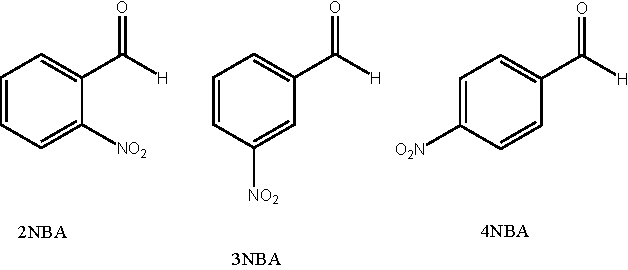
\includegraphics[width=\textwidth]{images/n-NBA.pdf}
\caption{Estructuras moleculares de 2-nitrobenzaldeh\'{i}do (2NBA), 3-nitrobenzaldeh\'{i}do (3NBA) y 4-nitrobenzaldeh\'{i}do (4NBA).}
\label{n-NBA}
\end{center}
\end{figure}

\end{frame}

\begin{comment}
Como parte del proceso de diseño e implementación  de software científico, es fundamental corroborar que los programas funcionan de forma correcta, por lo que se realizaron pruebas con moléculas que cuentan con entalpías de formación conocidas y que han sido reportadas en la literatura científica \cite{Ximello2020}. Las moléculas elegidas son isómeros del nitrobenzaladeído (figura \ref{n-NBA}) y son:

Los derivados de nitrobenzaladeh\'{i}do son compuestos aromáticos que tienen un gran número de aplicaciones. Entre ellos se encuentran los intermediarios en la preparación de productos químicos de alto valor agregado, pesticidas, materiales ópticos no lineales, productos farmacéuticos, bases de Schiff, etcétera \cite{Ximello2020}.
\end{comment}

%...................................................
%++++++++++++++++++++++++++++++++++++++++++++++++++++++++
%++++++++++++++++++++++++++++++++++++++++++++++++++++++++
%...................................................

\begin{frame}
\frametitle{Conjunto de pruebas: 2NBA, 3NBA y 4NBA}

\begin{table}[H]
\centering
\begin{tabular}{|c|c|c|}
\hline
	\multicolumn{3}{||c||}{$\enthalpy*(f){}(298.15 \mathrm{K})\; \mathrm{kJ\;mol^{-1}}$}\\
\hline
\hline
	n-NBA & Ximello \textit{et al.}[1] & EnthalpyTajti\\ 
\hline 
2NBAa & -28.19 & -28.19\\
\hline
2NBAb & -36.25 & -36.25\\ 
\hline 
3NBAa & -53.82 & -53.82\\
\hline
3NBAb & -55.46 & -55.46\\ 
\hline 
4NBAa & -53.84 & -53.84\\ 
\hline  
\end{tabular} 
	\caption{Entalpías de formación en fase gasesosa obtenidas mediante el método G4 de Gaussian de 2NBA, 3NBA y 4NBA a $T$ = 298 K y $p^{\circ}$ = 0.1 MPa, reportadas por Ximello \textit{et al.}}
\label{Ximello-table-1}
\end{table}
\textit{\tiny{[1] Ximello A., Ramos F., Rojas A., Hernández-Pérez J. M., Camarillo E. A., Solano-Altamirano J. M., Sandoval-Lira J., y Flores H., J. Chem. Eng. 65, 4935 (2020).}}
\end{frame}

\begin{comment}
Las entalpías de formación de las moléculas fueron calculadas utilizando los métodos G4 y G3MP2, así mismo, se utilizaron las aproximaciones de oscilador armónico/rotor rígido  y Nicolaides  en todas las moléculas. Para ello, las frecuencias se calcularon a un nivel teórico B3LYP/6-31G(2df,p) escaladas a 0.9854 y 0.89290. Las entalpías átomicas de formación  fueron a $T$ = 0 y sus correcciones térmicas a $T$ = 298 K se tomaron de la referencia \cite{NIST1998} (excluyendo el valor del átomo de Carbono, cuyo dato coincide con Tajti  para el método G4). Los archivos de salida proceden del software \textbf{Gaussian09}, mientras que el archivo que contiene la información necesaria para nuestro programa fue obtenida por el script \textbf{\textit{gendeltahfinputfile}} (proviente del \textbf{Laboratorio de Fisicoquímica Orgánica Teórica de la BUAP}). Los valores de la entalpía de formación a $T$ = 298 K calculados por nuestro programa del 2-nitrobenzaldehído (2NBA), 3-nitrobenzaldehído (3NBA) y 4-nitrobenzaldehído (4NBA) se muestran a continuación.
\end{comment}

%...................................................
%++++++++++++++++++++++++++++++++++++++++++++++++++++++++
%++++++++++++++++++++++++++++++++++++++++++++++++++++++++
%...................................................
\begin{frame}
\frametitle{Conjunto de pruebas: 2NBA, 3NBA y 4NBA}
\begin{table}[H]
\centering
\begin{tabular}{|c|c|c|}
\hline
	\multicolumn{3}{||c||}{$\enthalpy*(f){}(298.15 \mathrm{K})\; \mathrm{kJ\;mol^{-1}}$}\\
\hline
\hline
	n-NBA & Ximello \textit{et al.}[1] & EnthalpyNIST\\ 
\hline 
2NBAa & -36.42 & -36.42\\
\hline
2NBAb & -26.60 & -26.60\\ 
\hline 
3NBAa & -54.94 & -54.94\\
\hline
3NBAb & -53.19 & -53.19\\ 
\hline 
4NBAa & -52.91 & -52.91\\ 
\hline  
\end{tabular} 
	\caption{Entalpías de formación en fase gasesosa obtenidas mediante el método G3MP2 de Gaussian de 2NBA, 3NBA y 4NBA a $T$ = 298 K y $p^{\circ}$ = 0.1 MPa, reportadas por Ximello \textit{et al.} Obsérvese la segunda columna.}
\label{Ximello-table-2}
\end{table}
\textit{\tiny{[1] Ximello A., Ramos F., Rojas A., Hernández-Pérez J. M., Camarillo E. A., Solano-Altamirano J. M., Sandoval-Lira J., y Flores H., J. Chem. Eng. 65, 4935 (2020).}}
\end{frame}

%...................................................
%++++++++++++++++++++++++++++++++++++++++++++++++++++++++
%++++++++++++++++++++++++++++++++++++++++++++++++++++++++
%...................................................
\begin{frame}
\frametitle{Conjunto de pruebas: 2NBA, 3NBA y 4NBA}
\begin{table}[H]
\centering
\begin{tabular}{|c|c|c|}
\hline
	\multicolumn{3}{||c||}{$\enthalpy*(f){}(298.15 \mathrm{K})\; \mathrm{kJ\;mol^{-1}}$}\\
\hline
\hline
	n-NBA & Ximello \textit{et al.}[1] & EnthalpyArgonne\\ 
\hline
2NBAa & -35.01 & -35.01\\
\hline
2NBAb & -25.19 & -25.19\\ 
\hline 
3NBAa & -53.52 & -53.52\\
\hline
3NBAb & -51.78 & -51.78\\ 
\hline
4NBAa & -51.50 & -51.50\\ 
\hline  
\end{tabular} 
	\caption{Entalpías de formación en fase gasesosa obtenidas mediante el método G3MP2 de Gaussian de 2NBA, 3NBA y 4NBA a $T$ = 298 K y $p^{\circ}$ = 0.1 MPa, reportadas por Ximello \textit{et al.} Obsérvese la segunda columna.}
\label{Ximello-table-3}
\end{table}
\textit{\tiny{[1] Ximello A., Ramos F., Rojas A., Hernández-Pérez J. M., Camarillo E. A., Solano-Altamirano J. M., Sandoval-Lira J., y Flores H., J. Chem. Eng. 65, 4935 (2020).}}
\end{frame}


\begin{comment}
Las 15 pruebas preliminares también se realizaron con el fin de reconocer posibles errores en los resultados durante la ejecución de los programas \textbf{EnthalpyTajti}, \textbf{EnthalpyNIST} y \textbf{EnthalpyArgonne}. No obstante, lo anterior sirve para confirmar que las comparación con Ximello \textit{et al.} arroja datos con un alto nivel de precisión. Por esta razón, podemos ratificar la utilidad de nuestro programa para realizar cálculos que requieran un alto nivel de confiabilidad en los resultados teóricos. 
\end{comment}

%...................................................
%++++++++++++++++++++++++++++++++++++++++++++++++++++++++
%++++++++++++++++++++++++++++++++++++++++++++++++++++++++
%...................................................


%*************************************************************
\section{Conclusiones}
%*************************************************************
\begin{frame}
\frametitle{Conclusiones}

\begin{itemize}

\item Se creó un programa de cómputo científico que calcula entalpías de formación de compuestos orgánicos a \textit{T} = 298.15 K con correciones opcionales a la energía interna utilizando aproximaciones como Nicolaides \textit{et al.}, rotor rígido y oscilador armónico, empleando archivos de salida de Gaussian09.

\vspace{1cm}

\item Se implementaron otros métodos con un alto nivel de teoría y conjuntos de bases pequeñas, los cuales fueron: G3, G3MP2, CBS-APNO, CBS-QB3 y G4. De igual forma, se añadieron valores experimentales reportados por la comunidad científica: Tajti \textit{et al.}, NIST y Argonne.

\end{itemize}
\end{frame}
%...................................................
%++++++++++++++++++++++++++++++++++++++++++++++++++++++++
%++++++++++++++++++++++++++++++++++++++++++++++++++++++++
%...................................................

\begin{frame}
\frametitle{Conclusiones}
También, se lograron otros objetivos específicos:
\vspace{1cm}

\begin{itemize}
\item Los programas fueron diseñados para utilizarse a través de la línea de comandos en un sistema operativo de GNU/Linux, dando como resultado, una alta eficiencia en el flujo de trabajo.

\item Se implementó una programación orientada a objetos que fragmentó el código en partes independientes, permitiendo así, reciclar el código para proyectos futuros.
\end{itemize}
\end{frame}

\end{document}
   
%...................................................
%++++++++++++++++++++++++++++++++++++++++++++++++++++++++
%++++++++++++++++++++++++++++++++++++++++++++++++++++++++
%...................................................
%...................................................
%++++++++++++++++++++++++++++++++++++++++++++++++++++++++
%++++++++++++++++++++++++++++++++++++++++++++++++++++++++
%...................................................%...................................................
%++++++++++++++++++++++++++++++++++++++++++++++++++++++++
%++++++++++++++++++++++++++++++++++++++++++++++++++++++++
%...................................................

